\documentclass{article}
\usepackage{graphicx}
\usepackage{fitbox}
\usepackage{subfig}
\begin{document}

The use of fitbox with a subfigure.  Note that the optional argument
for the command counts the lines for the subcaptions.  

\SetFitboxLayout[1]{3}{2}




%\clearpage
\begin{figure}
  \centering
  \subfloat[First
  Vitruvian]{\fitbox*{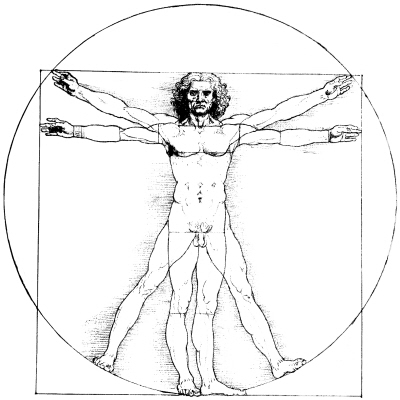
\includegraphics{vitruvian}}}%
  \subfloat[Second
  Vitruvian]{\fitbox*{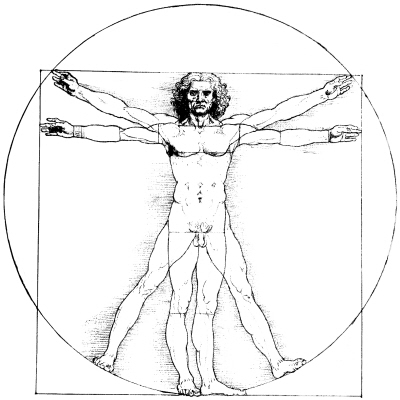
\includegraphics{vitruvian}}}\\
  \subfloat[Third
  Vitruvian]{\fitbox*{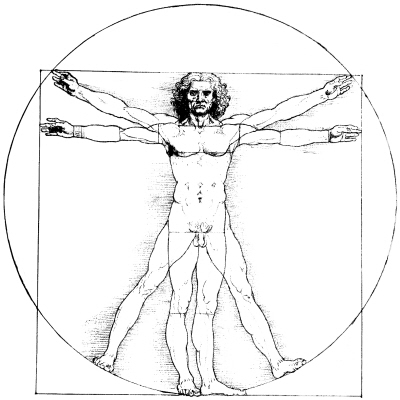
\includegraphics{vitruvian}}}%
  \subfloat[Fourth
  Vitruvian]{\fitbox*{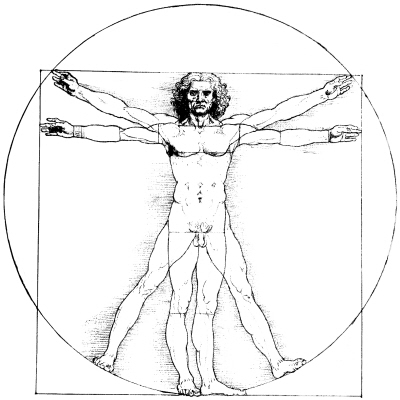
\includegraphics{vitruvian}}}\\
  \subfloat[Fifth
  Vitruvian]{\fitbox*{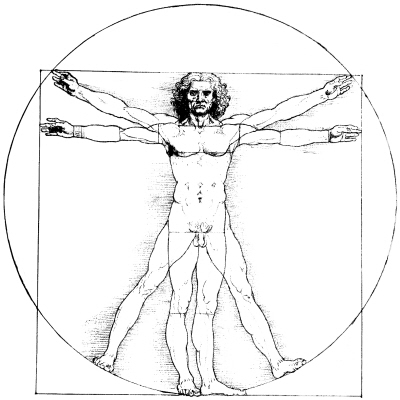
\includegraphics{vitruvian}}}%
  \subfloat[Sixth
  Vitruvian]{\fitbox*{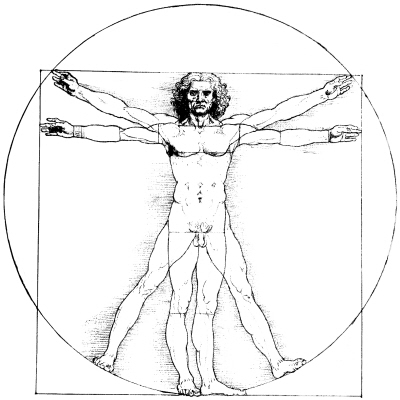
\includegraphics{vitruvian}}}
  \caption{Six Vitruvians}
  \label{fig:vitruvians}
\end{figure}

\SetFitboxLayout{3}{2}

%\clearpage
\begin{figure}
  \centering
  \subfloat{\fitbox*{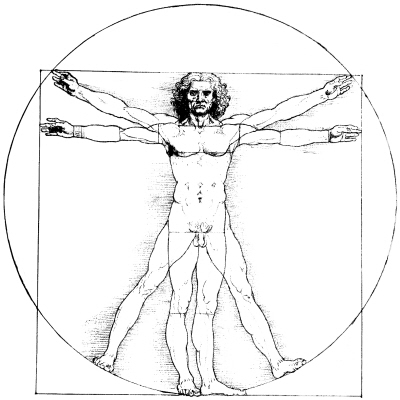
\includegraphics{vitruvian}}}%
  \subfloat{\fitbox*{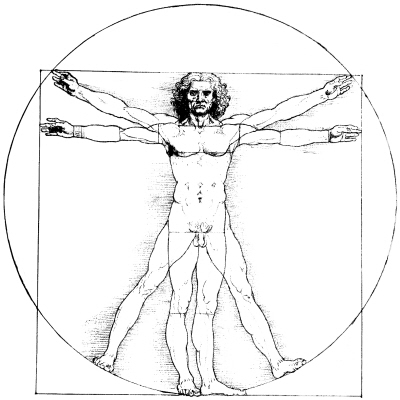
\includegraphics{vitruvian}}}\\
  \subfloat{\fitbox*{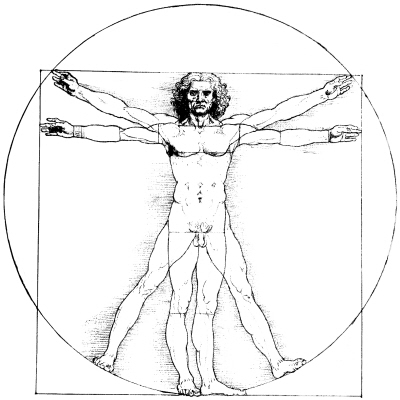
\includegraphics{vitruvian}}}%
  \subfloat{\fitbox*{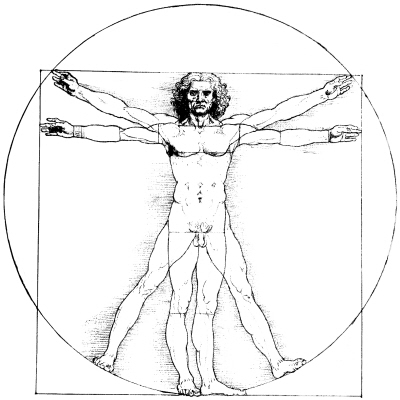
\includegraphics{vitruvian}}}\\
  \subfloat{\fitbox*{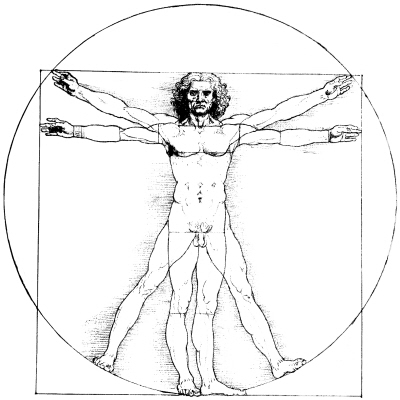
\includegraphics{vitruvian}}}%
  \subfloat{\fitbox*{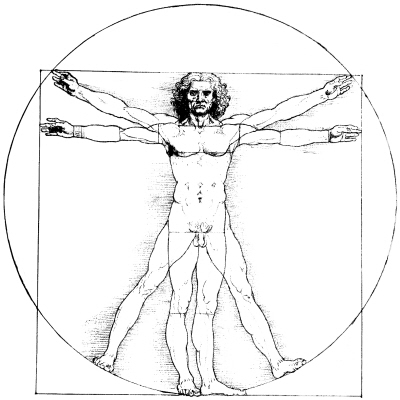
\includegraphics{vitruvian}}}
  \caption{Six Vitruvians, no subcaptions}
  \label{fig:vitruvians1}
\end{figure}


\end{document}
